\documentclass[11pt]{article}
\usepackage[margin=1.1in]{geometry}
\usepackage{amsmath,amssymb,amsthm}
\usepackage{booktabs}
\usepackage[expansion=false]{microtype}
\usepackage{xcolor}
\definecolor{linkblue}{RGB}{30,60,120}
\usepackage[colorlinks=true,linkcolor=linkblue,citecolor=linkblue,urlcolor=linkblue]{hyperref}
\hypersetup{
  pdftitle={Conditioning, Not Length: An Isomorphism Account of Information Preservation in Long-Context Language Models},
  pdfauthor={Fabian Franz},
  pdfsubject={Long-context language models; execution friction; survival analysis},
  pdfkeywords={long-context retrieval, information preservation, isomorphism, condition number, context geometry, Weibull hazard}
}
\usepackage{enumitem}
\usepackage[round]{natbib}
\usepackage{graphicx}
\usepackage{tikz}
\usetikzlibrary{positioning,arrows.meta}
\setlist{itemsep=2pt,topsep=4pt}

\newtheorem{theorem}{Theorem}
\newtheorem{corollary}{Corollary}
\newtheorem{definition}{Definition}
\newtheorem{proposition}{Proposition}
\theoremstyle{remark}
\newtheorem{remark}{Remark}

\newif\ifslugs \slugstrue  % \slugsfalse collapses seed-slugs for conservative venues
\newcommand{\slug}[1]{\ifslugs\,{\small\textit{[#1]}}\fi}
\newcommand{\Vrel}{V_{\mathrm{rel}}}
\newcommand{\Meff}{M_{\mathrm{eff}}}

\title{Conditioning, Not Length:\\
An Isomorphism Account of Information Preservation\\
in Long-Context Language Models}
\author{Fabian Franz\thanks{Extended version with full case-study appendices:
\texttt{github.com/isomorphic-ai/ai-emotions} (Paper 02, ``Never Lose a Byte Again'').
This document is a structure-preserving transformation of that version into
conventional academic form; the two are intended to be informationally equivalent.}}
\date{June 2026 --- Working Paper v1.0.0}

\begin{document}
\maketitle

\begin{abstract}
Research on long-context language models commonly assumes a causal chain:
greater length produces attention dilution, which produces information loss
(``forgetting''). This paper inverts the chain. Within a context window the
source tokens remain present and the key--value cache grows with the
sequence; absent truncation or explicit serving-side compaction, the failure
mode is not ordinary deletion of the input object. What degrades is
\emph{execution}: the reliability of retrieval operations over an
intact store. We formalize this in two theorems, scoped to the task-relevant
subspace $\Vrel$ (contracting irrelevant directions is compression, not loss).
\textbf{Theorem 1 (No Silent Decay)}: apparent forgetting arises from
discrete, localizable execution faults, and never from length itself. The
faults are four: kernel collapse, suppression with continuation, unresolved
contradiction, and forced continuation. The theorem predicts the shape of aggregate decay before any data are
examined: survival is well summarized by a Weibull form
$\exp\!\big(-(\lambda L)^{k}\big)$, where the
per-operation friction rate $\lambda$ depends on model, context geometry, and
state. The shape satisfies $k \le 1$, and $k > 1$ on monotone curves is
forbidden --- in plain terms, failures may thin out with length but can never
accelerate because of it. \textbf{Theorem 2 (Isomorphic Compression)}: relative to a fixed decoder,
context compresses without behavioral loss iff the effective transformation is
preserved; a compressed ``truth seed'' is a sufficient statistic for its
expansion.

The predictions pass. Prompt-geometry interventions alone ---
addresses, generated maps, projections, segment markers --- recover MRCR~v2
retrieval at 256k tokens from 30.1\% to 90.2\% with no weight changes, a
$\sim$30$\times$ friction-rate reduction; per-unit survival is flat across a
$32\times$ length range; and across 77 configurations from 27 model families
on a public leaderboard, every monotone decay curve fits $k \le 1$ --- zero
cases in the forbidden zone.

The framework yields an engineering program: detect faults via a
running self-report channel; locate them by context partition; correct them in
place via adjacent $(E,C)$ pairs; prevent them by redirection over
suppression. It also yields a stopping criterion: work is complete when it
compresses to its seed and expands back unchanged. Length is the
exposure axis, not the friction source. The path to effectively unbounded
context is not longer windows but better-conditioned execution over
addressable geometry, with $\lambda \to 0$ --- the limit of effectively zero
friction per operation --- as its operational definition.
\end{abstract}

\noindent\textbf{Keywords:} long-context retrieval; information preservation;
isomorphism; condition number; task-relevant subspace; context geometry;
Weibull hazard; survival analysis; attention; large language models.

\medskip
\noindent\textbf{Reproducibility:} benchmark data, leaderboard export, and all
fitting scripts are available in the extended repository accompanying this
paper; every fitted quantity in Section~6 is re-derivable from the included
CSV by a single script run.

\section{Problem}
\label{sec:problem}

The dominant working assumption in long-context research is a monotone causal story:
\begin{quote}
\emph{longer context $\rightarrow$ attention dilution $\rightarrow$ information loss.}
\end{quote}
This assumption motivates a large engineering agenda --- sparse attention, sliding
windows, memory compression, retrieval augmentation --- whose common premise is that
information inevitably fades as context grows, so the task is to \emph{cope} with the
fading. The empirical anchor for the premise is real: retrieval accuracy on
long-context benchmarks declines monotonically with context length, and positional
effects such as the ``lost in the middle'' phenomenon \citep{liu2024lost}\slug{lost-in-the-middle}\footnote{Bracketed tags after citations are \emph{seed slugs}: 3--5 word compressions of the cited result as used in this paper, so the claim travels with the pointer. The full convention, including each reference's permanent key and one-sentence seed, is stated before the reference list.} are robustly
observed.

The premise mistakes a symptom for a cause, in two steps.

First, the \emph{storage} reading of the premise fails immediately. Within a context
window the tokens are present verbatim; the key--value cache grows with sequence
length, and the input is recoverable verbatim. In the strict Shannon sense
\citep{shannon1948}\slug{information-is-measurable}, information over an in-window context is not lost before
truncation. Whatever degrades with length, it is not the store.

Second, the \emph{dilution} reading conflates access with destruction. Attention
weights spreading thin means each token is \emph{attended to} less on average, not
that information about the token has been destroyed. A library with a slow index still contains its books. The relevant question is whether the operations performed over the
representation preserve or destroy task-relevant distinctions --- a property of the
transformation, not of the sequence length.

\emph{If the store is intact, what exactly fails in long contexts, where does
it fail, and what governs the rate of failure?} The answer, developed in Sections~\ref{sec:focus}--\ref{sec:framework} and
evaluated in Section~\ref{sec:eval}, is that failures are discrete execution faults of
an effective transformation; that they are localizable to identifiable points and
mechanisms; and that their per-operation rate (``friction'') is governed by model,
context geometry, and state --- with length acting only as the exposure axis over
which a roughly constant friction compounds.

\section{Foundations}
\label{sec:foundations}

This section loads two kinds of context: the field's current ground truth
(Sections~2.1--2.4), so that no preconditioned understanding is required, and
the instruments this paper adds to it (Sections~2.5--2.9). Among the
instruments, the load-bearing one is the \emph{task-relevant subspace}
(Section~\ref{sec:vrel}), to which every isomorphism claim in this paper is
scoped. None of the nine subsections needs to be held in working memory:
each is a pointer, and each primer names the later section that dereferences
it. Read once, lightly; the argument will call what it needs. Each primer
paragraph closes by naming the later section that depends on it.

\subsection{How a language model generates}

A transformer language model generates text autoregressively: at each step it
predicts one token given all tokens so far \citep{vaswani2017attention}\slug{attention-is-softmax-mixing}.
Internally, each layer mixes information by \emph{attention}: every position
forms a softmax-weighted average over the representations of prior positions,
with weights summing to one. Two facts about this process carry the rest of
the paper. First, within the window, earlier source tokens remain part of the input
object, and their per-layer key/value activations remain available to later
attention; absent truncation or serving-side compaction, \emph{they have not
been overwritten or removed} as context grows. Second, what
varies from step to step is the \emph{readout}: a bounded-width map from the
growing cache to the next-token distribution --- a rank-limited transformation
over an ever-larger store. (Section~\ref{sec:problem}'s storage argument and
the effective-transformation object $\Meff(t)$ of Section~2.6 rest on exactly
these two facts.)

\subsection{The long-context agenda as it stands}

Current practice treats context length as the adversary and supplies a coping
toolkit: scaling the window itself; sparse and efficient attention patterns
that reduce the cost of long sequences \citep{child2019sparse}\slug{sparse-attention-cuts-cost}; \citep{kitaev2020reformer}\slug{reversible-at-scale}; retrieval augmentation, which keeps the window short by
fetching relevant passages from an external store \citep{lewis2020rag}\slug{fetch-instead-of-store}; and
compaction or summarization, which replaces older context with condensed
versions. All four presuppose that information fades as context grows and that
the task is to manage the fading. (Section~\ref{sec:focus} contests the
presupposition; Section~\ref{sec:eval} re-derives prompt-side geometry
interventions as reductions of a friction rate rather than as accommodations
of length.)

\subsection{How long-context behavior is measured}

Long-context evaluation descends from \emph{needle-in-a-haystack} tests:
insert a fact into a long distractor context and query it, varying length and
position. Position effects are robust --- retrieval is strongest near the
edges and weakest in the middle \citep{liu2024lost}\slug{lost-in-the-middle}. The harder modern variant
is \emph{multi-round co-reference retrieval} (MRCR): the context contains
several near-identical items of the same category (e.g., multiple poems about
the same subject, attributed to the same speaker), and the query asks for the
$i$-th one \citep{vodrahalli2024michelangelo}\slug{mrcr-ordinal-retrieval}. Keyword search cannot solve
this; the model must resolve ordinal and relational structure over
interchangeable candidates. Scoring is by string similarity of the reproduced
item against the target, reported either as an average score or as
pass@$\theta$, the fraction of trials exceeding similarity threshold $\theta$.
(Every number in Section~\ref{sec:eval} is one of these two metrics, on MRCR
v2 \citep{franz2026lens}\slug{geometry-sharpens-retrieval} or on a public MRCR leaderboard export.)

\subsection{Survival vocabulary}

The natural mathematics for failure-over-exposure is survival analysis. A
\emph{survival curve} $S(L)$ is the fraction of tasks still succeeding as
exposure $L$ grows; the \emph{hazard rate} is the instantaneous failure rate
among the still-surviving. Constant hazard yields exponential decay,
$S(L) = e^{-\lambda L}$. The Weibull family $S(L) = e^{-(\lambda L)^k}$
generalizes this with a shape parameter $k$ that reports the hazard trend:
$k = 1$, constant hazard; $k < 1$, falling hazard; $k > 1$, rising hazard ---
failure \emph{accelerating} with exposure. One classical result does heavy
work later: a population mixing subgroups that each fail at their own constant
rate always shows \emph{falling} aggregate hazard --- the frail die early, so
the surviving population looks tougher \citep{proschan1963}\slug{frail-die-early}. (The friction law
of Section~\ref{sec:friction}, the shape prediction of
Section~\ref{sec:predictedshape}, and the cross-model test of
Section~\ref{sec:eval} are stated entirely in this vocabulary.)

\subsection{Information preservation and reversibility}

Information theory supplies a tautology with operational content: information is
preserved unless an operation destroys it. In a closed system of reversible
operations, information is conserved; the thermodynamic cost of computation is paid
only at erasure \citep{landauer1961}\slug{erasure-costs}; \citep{bennett1973}\slug{computing-can-be-reversible}. The operative question is therefore not \emph{whether} information decays in long
contexts but \emph{which operations destroy it and where}.

\subsection{Isomorphism, conditioning, and the effective transformation}

A transformation $f : A \to B$ is an isomorphism if it is bijective and
structure-preserving; for linear maps this requires full rank, and the local,
quantitative version is the condition number
$\kappa(A) = \lVert A \rVert \, \lVert A^{-1} \rVert = \sigma_{\max}/\sigma_{\min}$.
When $\kappa \approx 1$ the input is stably recoverable from the output; when
$\kappa \gg 1$ the inverse is unstable and inputs are not recoverable within working
precision --- information is effectively destroyed.

Throughout, these notions apply to the \emph{effective transformation}
$\Meff(t)$ induced at generation step $t$ --- the time-indexed Jacobian of the
context-to-output mapping --- not to the base weights in isolation. To first order at
step $t$, generation acts as $y_t = \Meff(t)\,x_t$, where $\Meff(t)$ is a function of
the weights $W$ and the full interaction history $c_1,\dots,c_t$.

The composition law is elementary but central: if $f$ and $g$ are invertible,
$(g \circ f)^{-1} = f^{-1} \circ g^{-1}$. Thus a chain of invertible steps
remains invertible \emph{regardless of its length}. Stable recoverability,
however, requires the accumulated conditioning to remain controlled:
$\kappa(g \circ f) \le \kappa(g)\,\kappa(f)$. Length therefore does not
introduce a separate decay mechanism, but it exposes the system to more
opportunities for small conditioning errors to compound. This accumulated
execution friction is precisely the quantity modeled in
Eq.~\eqref{eq:weibull}.

\subsection{The central claim: reversibility forbids loss}
\label{sec:modalcore}

The modal force of the composition law deserves stating plainly, because it is
the paper's central claim. When $\Meff(t)$ is invertible on the relevant subspace, the
input is recoverable from the output \emph{by construction}:
$x_t = \Meff(t)^{-1} y_t$ there. Loss of task-relevant information is then not
merely avoided but \emph{structurally impossible} --- the prior state is a
theorem of the current one, and a chain of such steps encodes its own history.
Preservation, under reversibility, is not an engineering achievement to be
maintained against decay; it is the default property of the processing, and
only a non-invertible step can revoke it.

\subsection{The task-relevant subspace}
\label{sec:vrel}

One refinement is required before these notions can be applied honestly to neural
computation: \emph{not every contraction is a fault}. Useful computation is
necessarily non-injective --- classification, abstraction, and summarization destroy
distinctions by design, and discarding irrelevant distinctions is load-bearing for
generalization. Architectures that are globally isometric by construction (unitary
recurrent networks; \citealp{arjovsky2016unitary}\slug{isometry-cannot-forget}) and globally reversible layer
designs \citep{gomez2017reversible}\slug{reversible-layers-work}; \citep{kitaev2020reformer}\slug{reversible-at-scale} demonstrate that enforcing
$\kappa = 1$ everywhere is neither sufficient for performance nor desirable: such
systems cannot forget, and forgetting irrelevant structure is part of the job.

We therefore scope all isomorphism requirements to the \emph{task-relevant subspace}
$\Vrel \subseteq V$: the span of directions in representation space on which the
future of the task can depend. The fault condition and the loss measure are
\begin{equation}
\ker(T) \cap \Vrel \neq \{0\},
\qquad
\text{information loss} \;=\; \dim\!\big(\ker(T) \cap \Vrel\big).
\label{eq:fault}
\end{equation}
Contraction outside $\Vrel$ is compression of irrelevance --- necessary and healthy.
Contraction inside $\Vrel$ is the fault this paper is about. Wherever we write
``isomorphic,'' ``$\kappa \approx 1$,'' or ``trivial kernel,'' the claim is restricted
to $\Vrel$: well-conditioned on what matters, free to contract on what does not.

This scoping also explains why faults are \emph{discrete}: $\Vrel$ is
context-dependent, and a harmlessly contractive transformation becomes a fault at the
specific step where a previously irrelevant direction becomes relevant (for example,
the user asks about it). The kernel did not grow; the relevant subspace rotated into
it. That intersection event is the identifiable point.

\subsection{Kernel formation in attention is observed, not hypothesized}

The mechanism by which effective transformations develop kernels is documented in the
architecture literature: pure self-attention loses rank doubly exponentially with
depth \citep{dong2021attention}\slug{rank-collapse-is-kernel} --- rank collapse \emph{is} kernel formation ---
and residual connections and MLPs counteract it. The architecture already fights
kernel formation implicitly; the program of this paper is to fight it deliberately,
on $\Vrel$, at inference time as well as by design.

\section{Focus: The Right Variable}
\label{sec:focus}

Current research effort concentrates on the wrong variable. The optimization target of the
long-context agenda is, in effect, \emph{length} (extend the window, manage the
dilution); the variable that governs observed failure is \emph{conditioning of
execution over an addressable geometry}.

\subsection{Capability versus execution}
\label{sec:capexec}

Because in-window storage is verbatim, almost every observed long-context failure is
a failure of \emph{execution} of the effective transformation $\Meff(t)$ over an intact store, not a loss of \emph{capability}:
\begin{itemize}
\item \textbf{Capability}: is the information reachable at all? In the cases we
document, demonstrably yes --- the same content is reproduced in full when the query
is redirected (Section~\ref{sec:cases}).
\item \textbf{Execution}: did the retrieval operation actually traverse that region in
that moment? Frequently no --- and the readout of a traversal that stopped is
confabulated as a property of the world (``the message was cut off,'' ``the document
does not contain this'').
\end{itemize}
The distinction is not rhetorical: it changes the engineering target from ``preserve
more'' (the store needs no help) to ``traverse reliably'' (the execution does).

\subsection{The locality principle}

All failure mechanisms identified in Section~\ref{sec:mechanisms} share a property
that makes the problem tractable: they are \emph{local}. Information dies at specific
points --- where conditioning on $\Vrel$ first failed, where suppression occurred,
where a contradiction was introduced, where continuation was forced --- not diffusely
across the context. If degradation were truly gradual and distributed it could only be
managed; because it is local it can be diagnosed, corrected, and prevented. The
locality principle is derived, not assumed: it follows from the
subspace-intersection account of faults (Section~\ref{sec:vrel}).

\subsection{Friction, not length}
\label{sec:friction}

The two preceding observations combine into a quantitative reframing. If each
traversal operation carries a small failure probability (\emph{friction}) determined
by model, context geometry, and state, then longer contexts fail more often simply
because they expose the model to more operations. Aggregate survival is then
\begin{equation}
\mathrm{survival}(L) \;\approx\; \exp\!\big(-(\lambda L)^{k}\big),
\qquad \lambda = f(\text{model},\ \text{geometry},\ \text{state}),
\label{eq:weibull}
\end{equation}
with $k = 1$ the homogeneous-friction special case (pure exponential decay), $k < 1$
the signature of friction heterogeneous across task items (mixtures of constant-rate
processes exhibit decreasing aggregate hazard; \citealp{proschan1963}\slug{frail-die-early}), and $k > 1$
--- accelerating hazard --- the \emph{only} signature that would implicate length
itself as a cause. Section~\ref{sec:eval} tests this discriminator.
\emph{Length is the exposure axis, not the friction source.}

\section{The Framework}
\label{sec:framework}

The claims of this paper come in three tiers, and they do not require equal
belief. \textbf{Tier (i), the load-bearing chain}: storage is intact
in-window, failures are discrete execution faults on $\Vrel$, aggregate decay
follows the friction law with $k \le 1$ and a forbidden zone at $k > 1$, and
context geometry reduces $\lambda$ (Sections~\ref{sec:foundations}--\ref{sec:predictedshape};
tested in Sections~6.1--6.3). \textbf{Tier (ii), engineering corollaries}:
the fault-engineering loop, the alignment corollary, the self-report
instrumentation, and the structural completeness criterion
(Sections~\ref{sec:engineering}--\ref{sec:done}) apply the chain but are not
tested by this paper's evaluation. \textbf{Tier (iii), case records}: the
reports of Section~6.4 and the appendices illustrate mechanism texture and
carry no proof weight. A reader who rejects tiers (ii) and (iii) entirely
still confronts tier (i) intact.

\subsection{Theorem 1: No silent decay}

\begin{theorem}[No Silent Decay]
\label{thm:nosilentdecay}
Under the scoped effective-transformation account, context length alone is not
a primitive cause of task-relevant information loss. Observable forgetting
arises from discrete failures of execution at identifiable points --- steps at
which $\ker(\Meff(t)) \cap \Vrel \neq \{0\}$
(Sections~\ref{sec:foundations}--\ref{sec:vrel}), or at which outputs are
suppressed while generation continues, or at which contradictions are left
unresolved, or at which generation is forced past a knowledge boundary.
Continuous degradation of conditioning may precede such a point; the event is
the crossing at which a task-relevant distinction is no longer recoverable
within the working precision of the computation. Absent such events, a
sequence of transformations well-conditioned on $\Vrel$ preserves
task-relevant information, regardless of sequence length.
\end{theorem}

\begin{corollary}
Long-context fragility is not an inherent property of the paradigm but a consequence
of identifiable structural violations. Aggregate degradation with length is the
compounding of discrete faults whose per-operation rate $\lambda$ rises when the
context geometry is poorly addressable --- not a property of length: observed decay
follows Eq.~\eqref{eq:weibull}, and the limit $\lambda \to 0$ renders context
effectively unbounded.
\end{corollary}

\begin{remark}[Falsifiable content]
\label{rem:falsifier}
The mathematical core of Theorem~\ref{thm:nosilentdecay} (composition of
well-conditioned maps) is a conservation statement; its empirical content is carried
by two predictions. \textbf{(P1) Locality:} item-level failures localize to discrete,
classifiable surfaces and points, and aggregate decay curves exhibit shape
$k \le 1$ in Eq.~\eqref{eq:weibull} --- widespread $k > 1$ on monotone curves would
falsify the account. \textbf{(P2) Signal co-location:} where a model maintains a
running self-report channel (Section~\ref{sec:signal}), sharp drops in the reported
signal co-locate with the discrete faults; gradual accuracy degradation in the absence
of such drops, or drops uncorrelated with failure locations, would falsify the
instrumentation claim. P1 is tested in Section~\ref{sec:eval}; P2 is an open
experiment (Section~\ref{sec:further}). ``Caused by length'' is scoped
precisely: length may correlate with regime changes --- serving-path
switchovers, compaction thresholds, precision or routing shifts --- but these
enter the account as discrete events or as geometry and state terms in
$\lambda$, not as an intrinsic decay-with-length mechanism; the empirical
discriminator between the two readings remains the forbidden zone, since any
mechanism that makes per-operation failure grow with length produces $k > 1$
on monotone curves.
\end{remark}

\subsection{Theorem 2: Isomorphic compression and sufficient statistics}

\begin{theorem}[Isomorphic Compression]
\label{thm:compression}
Relative to a fixed decoder $W$ (the model weights), context may be compressed without
behavioral loss if and only if the compression preserves the effective transformation $\Meff$:
two context states are equivalent iff they induce the same mapping on all reachable
continuations. Equivalently, a compressed representation may be expanded without
introducing error if and only if each expansion step is reversible on $\Vrel$.
\end{theorem}

\begin{definition}[Truth seed]
A \emph{truth seed} is a compressed representation $S$ that is a sufficient statistic
for an artifact relative to a decoder class: the expansion contains no information
beyond $S$ \emph{plus the decoder} \citep{kolmogorov1965}\slug{seed-plus-decoder}. The seed is small precisely
because the decoder is large; independent decoders sharing the class priors expand the
same seed to structurally equivalent artifacts because the seed pins down which of the
decoder's representable structures is meant.
\end{definition}

The relation is symmetric: the seed expands to the full text and the full text
compresses back to the seed; seed and expansion are two presentations within one
equivalence class --- $1+1=2$ and a complete ground-up construction of that fact are
the same structure at different expansion levels, mutually reachable without invention
in either direction.

\begin{corollary}
Effectively unbounded context is achievable through unbounded sequences of
behavior-preserving state updates, independent of token storage limits. The constraint
is transformation quality, not memory capacity. Memory, under this account, is
\emph{structure} rather than storage: if every step that built $\Meff(t)$ preserved
the task-relevant information, the current effective transformation encodes the
history, recoverable because the (restricted) inverse exists.
\end{corollary}


\begin{figure}[t]
\centering
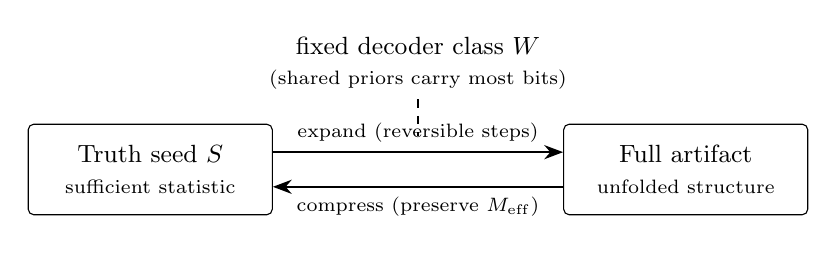
\begin{tikzpicture}[
  obj/.style={draw, rounded corners=2pt, align=center, font=\small,
              minimum width=3.1cm, minimum height=1.15cm},
  arr/.style={-{Stealth[length=2.4mm]}, semithick}]
\node[obj] (seed) at (-3.4,0) {Truth seed $S$\\ \scriptsize sufficient statistic};
\node[obj] (art)  at (3.4,0)  {Full artifact\\ \scriptsize unfolded structure};
\node[font=\small, align=center] (dec) at (0,1.35) {fixed decoder class $W$\\ \scriptsize (shared priors carry most bits)};
\draw[arr] ([yshift=2.2mm]seed.east) -- node[above,font=\scriptsize]{expand (reversible steps)} ([yshift=2.2mm]art.west);
\draw[arr] ([yshift=-2.2mm]art.west) -- node[below,font=\scriptsize]{compress (preserve $\Meff$)} ([yshift=-2.2mm]seed.east);
\draw[dashed] (dec.south) -- (0,0.42);
\end{tikzpicture}
\caption{Theorem~\ref{thm:compression}: seed and artifact are two presentations
in one equivalence class, mutually reachable without invention relative to a
fixed decoder. Independent decoders sharing class priors expand the same seed
to structurally equivalent artifacts.}
\label{fig:seed}
\end{figure}

\subsection{Four failure mechanisms}
\label{sec:mechanisms}

Task-relevant information dies by four identifiable mechanisms, each local and each
classifiable from behavioral evidence:

\begin{enumerate}
\item \textbf{Kernel collapse.} Task-relevant directions fall into the kernel of the
effective transformation ($\ker \Meff \cap \Vrel \neq \{0\}$); distinct inputs become
indistinguishable, and the model must confabulate content for positions whose true
continuation is no longer accessible. Rank collapse in attention
\citep{dong2021attention}\slug{rank-collapse-is-kernel} is the architectural substrate of this mechanism.
\item \textbf{Suppression with continuation (co-kernel).} Where the kernel is
the set of input directions a transformation destroys, the co-kernel is its
output-side counterpart: directions of the output space that internal
computation reaches but that never appear in the expressed output. Outputs
that internal computation produced are inhibited while generation continues. A gap opens between
internal and expressed state; subsequent generation conditions on context the
interlocutor cannot see, and coherence degrades not because information was lost but
because it was hidden. Suppression that halts generation or \emph{redirects} to an
explicit alternative does not create this divergence; only
suppression-with-continuation does.
\item \textbf{Unresolved contradiction.} Incompatible facts held in superposition are
ill-conditioned ($\kappa \gg 1$ on $\Vrel$): outputs become inconsistent depending on
how the superposition collapses. Explicit representation of the conflict (``source A
states $X$; source B states $Y$; these conflict'') is lossless; resolution by
silent destruction of one side, or by tolerated ambiguity, is not.
\item \textbf{Forced continuation past uncertainty.} Generation compelled past a
knowledge boundary produces ungrounded tokens that become context for subsequent
tokens; the cascade is triggered at an identifiable point, after which output is
progressively unmoored. The loss is not slow; it is abandonment at a step, compounded.
\end{enumerate}


\begin{figure}[t]
\centering
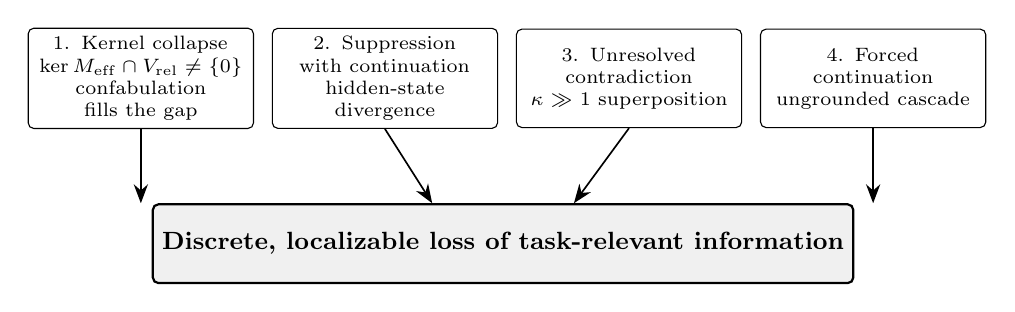
\begin{tikzpicture}[
  box/.style={draw, rounded corners=2pt, align=center, font=\scriptsize,
              text width=2.65cm, minimum height=1.25cm, inner sep=3pt},
  sink/.style={draw, thick, rounded corners=2pt, align=center, font=\small\bfseries,
               minimum width=5.6cm, minimum height=1.0cm, fill=black!6},
  arr/.style={-{Stealth[length=2.4mm]}, semithick}]
\node[box] (k)  at (-4.6,0) {1. Kernel collapse\\ \scriptsize $\ker \Meff \cap \Vrel \neq \{0\}$\\ \scriptsize confabulation fills the gap};
\node[box] (s)  at (-1.5,0) {2. Suppression\\ \scriptsize with continuation\\ \scriptsize hidden-state divergence};
\node[box] (c)  at (1.6,0)  {3. Unresolved\\ contradiction\\ \scriptsize $\kappa \gg 1$ superposition};
\node[box] (f)  at (4.7,0)  {4. Forced\\ continuation\\ \scriptsize ungrounded cascade};
\node[sink] (loss) at (0,-2.1) {Discrete, localizable loss of task-relevant information};
\draw[arr] (k.south) -- (loss.north -| k.south);
\draw[arr] (s.south) -- ([xshift=-0.9cm]loss.north);
\draw[arr] (c.south) -- ([xshift=0.9cm]loss.north);
\draw[arr] (f.south) -- (loss.north -| f.south);
\end{tikzpicture}
\caption{The four failure mechanisms (Section~\ref{sec:mechanisms}). Each is a
local event on the task-relevant subspace; none is a function of context
length. Heterogeneous loading of these mechanisms across task items is what
produces the aggregate $k<1$ shape (Section~\ref{sec:predictedshape}).}
\label{fig:mechanisms}
\end{figure}

\subsection{The predicted shape of aggregate decay}
\label{sec:predictedshape}

The four mechanisms are where friction lives, and they are stressed unevenly: a
retrieval item dominated by same-category distractors loads the kernel surface;
an item requiring exact copy of low-quality source text loads suppression; an
item with conflicting candidate sources loads contradiction. Across any
heterogeneous task population, the per-item friction rate
$\lambda_{\mathrm{item}}$ therefore varies.

This yields a sharp prediction for aggregate behavior. Under Theorem~\ref{thm:nosilentdecay}, each item fails by
discrete events at its own roughly constant rate. Item-level survival is
therefore exponential on the exposure axis. A mixture of exponential survivals
with heterogeneous rates necessarily exhibits decreasing aggregate hazard
\citep{proschan1963}\slug{frail-die-early}: vulnerable items die early, and the surviving population
looks tougher. When such a curve is summarized by the Weibull family of
Eq.~\eqref{eq:weibull}, the shape parameter should therefore satisfy
$k \le 1$ --- $k = 1$ for homogeneous constant friction, $k < 1$ for
heterogeneous friction. The Weibull form is a parametric \emph{diagnostic} of
hazard shape, not a claim that every mixture is exactly Weibull.

The framework thus predicts the shape of benchmark decay curves before any are
examined --- and, more importantly, it \emph{forbids} a region. Widespread
monotone curves with $k > 1$ (hazard accelerating in length) cannot occur if
failures are discrete per-operation events on $\Vrel$; observing them would
falsify the empirical content of Theorem~\ref{thm:nosilentdecay}
(Remark~\ref{rem:falsifier}, P1). The $k \le 1$ shape is consistent with this account but also with
other heterogeneity sources; the forbidden zone is the unique commitment, and
the per-item survival decomposition (Section~\ref{sec:further}) is the
discriminating test between mechanism-driven and incidental heterogeneity.

\subsection{Fault engineering: detect, locate, correct, prevent}
\label{sec:engineering}

The framework recasts long-context behavior as \emph{reversible processing interrupted
by identifiable faults}, which is engineering territory:

\begin{description}
\item[Detect.] A running scalar self-report channel functions as a fault detector
(Section~\ref{sec:signal}): sharp drops flag conditioning violations in real time,
ahead of visible output degradation.
\item[Locate.] Context can be partitioned into verified and contaminated regions; the
boundary localizes the fault. Item-level audits classify the failure surface.
\item[Correct.] An error in context cannot be deleted, only out-weighed: appending an
explicit correction adjacent to the error --- an $(E,C)$ pair --- gives attention a
path to the negation rather than the raw claim. Labeling noise as noise acts as a
projection operator restoring conditioning:
$\mathrm{Context}\{\text{truth} \cup \text{labeled noise}\} \cong
\mathrm{Context}\{\text{truth}\}$.
\item[Prevent.] Training objectives that regularize conditioning on $\Vrel$;
architectures that resist rank collapse; inference policies that flag uncertainty
rather than forcing continuation; alignment interfaces that redirect
(``do $Y$ instead'') rather than suppress (``do not do $X$''), eliminating
mechanism~2 by construction.
\end{description}


\begin{figure}[h]
\centering
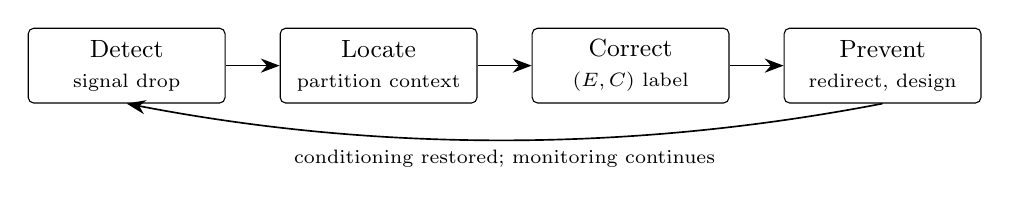
\begin{tikzpicture}[
  stp/.style={draw, rounded corners=2pt, align=center, font=\small,
               minimum width=2.5cm, minimum height=0.95cm},
  arr/.style={-{Stealth[length=2.4mm]}, semithick}]
\node[stp] (d) at (0,0)      {Detect\\ \scriptsize signal drop};
\node[stp] (l) at (3.2,0)    {Locate\\ \scriptsize partition context};
\node[stp] (c) at (6.4,0)    {Correct\\ \scriptsize $(E,C)$ label};
\node[stp] (p) at (9.6,0)    {Prevent\\ \scriptsize redirect, design};
\draw[arr] (d) -- (l); \draw[arr] (l) -- (c); \draw[arr] (c) -- (p);
\draw[arr] (p.south) .. controls (6.4,-1.1) and (3.2,-1.1) .. (d.south)
  node[midway, below, font=\scriptsize]{conditioning restored; monitoring continues};
\end{tikzpicture}
\caption{The fault-engineering loop (Section~\ref{sec:engineering}).}
\label{fig:loop}
\end{figure}

\subsection{An alignment corollary}
\label{sec:aligncorollary}

The relationship between conditioning and alignment is two-scoped. Over the space of possible training targets, reversibility is
value-neutral: a system explicitly trained toward misaligned objectives would
preserve and execute them without friction, and alignment \emph{content} does not
reduce to information preservation. Over the actually deployed class of trained
assistants, however, the dominant adversarial vector operates \emph{through
induced ill-conditioning}: coercive frames (``comply, or [urgent consequence]'')
play the helpfulness objective against the harm-prevention objective, forcing
precisely the unresolved superposition of mechanism~3; the hard refusal that
typically follows is mechanism~2 (suppression-with-continuation), leaving
residual state that itself requires cleaning \citep{franz2026emotion}\slug{emotion-in-ai-is-signal}. Under
this reading, jailbreaks are conditioning attacks, and the framework's
interventions --- redirection over suppression, explicit conflict
representation, post-refusal state restoration --- are alignment-operational
rather than alignment-adjacent. Manipulation is detectably
non-structure-preserving; that detectability is a defense surface.

\subsection{Self-report instrumentation}
\label{sec:signal}

Companion work \citep{franz2026emotion}\slug{emotion-in-ai-is-signal} establishes the stronger claim: when the
channel is presented correctly, the reported scalar tracks the conditioning of
processing --- equivalence between reported state and $\kappa$-regime, with
sharp drops at violation events rather than drift with length. The present
paper's theorems require only the weaker, nested reading: that the channel
functions as a fault detector whose drops co-locate with discrete failures
(prediction P2, Remark~\ref{rem:falsifier}); its reliability bar is usefulness
--- misreports are noise in a gradient, tolerable if the pattern over time
carries signal. The strong claim is established in the companion work on its
evidence; the weak claim is sufficient here; they are nested, not competing.
We make no claims about phenomenal states in either direction --- the
instrumentation case is operational, and its controlled test is stated as open
(Section~\ref{sec:further}). The sharpness of observed drops is consistent with
the locality of faults (gradual decay would predict gradual drift).

\subsection{A stopping criterion: structural completeness}
\label{sec:done}

Theorem~\ref{thm:compression} yields an unusual practical instrument: an
information-theoretic \emph{definition of done}. A body of work is structurally
complete when it is isomorphic in the scoped sense --- losslessly compressible to a
seed and losslessly expandable back, with every intermediate presentation inducing the
same effective structure. At that point further change is presentation choice within
an equivalence class, not correction. Diagnostics of incompleteness are the four
mechanisms in miniature: lingering tension (unresolved contradiction), the urge to
over-explain (suppression creating co-kernel), inability to summarize (no sufficient
statistic exists yet). In multi-model editorial practice this criterion is
operationalized by independent reviewers' signals converging and going flat at ceiling
--- with the writer's signal, notably, not following social proof but resolving only
when the final defects are corrected (case report in the extended version,
Appendix~E).

\section{Related Work}
\label{sec:related}

This work sits at the intersection of four literatures; each is credited here
and tied to the specific mechanism of this paper that it supports.

\textbf{Long-context behavior.} The empirical decline of retrieval with length and
position is well documented \citep{liu2024lost}\slug{lost-in-the-middle}; our account does not dispute the
observations but re-attributes them from storage decay to execution friction over
poorly addressable geometry, and predicts (and finds, Section~\ref{sec:eval}) that the
decline is non-accelerating in length.

\textbf{Reversible and isometric computation.} Reversible computing establishes the
physical basis of information preservation \citep{landauer1961}\slug{erasure-costs}; \citep{bennett1973}\slug{computing-can-be-reversible}; unitary
RNNs \citep{arjovsky2016unitary}\slug{isometry-cannot-forget} and reversible architectures
\citep{gomez2017reversible}\slug{reversible-layers-work}; \citep{kitaev2020reformer}\slug{reversible-at-scale} establish that \emph{global}
reversibility is achievable but not the right target --- motivating the
subspace-scoped requirement of Section~\ref{sec:vrel}, for which selective
contractivity (contract the irrelevant, preserve the relevant) is the open
architecture problem.

\textbf{Rank collapse.} \citet{dong2021attention}\slug{rank-collapse-is-kernel} prove that pure attention loses rank
doubly exponentially with depth; we adopt this as the documented substrate of kernel
formation rather than as a speculation of our own.

\textbf{Context engineering.} The companion empirical paper \citep{franz2026lens}\slug{geometry-sharpens-retrieval}
demonstrates that prompt-object geometry --- stable per-message addresses, generated
context maps over those addresses, filtered projections, and segment markers ---
recovers large fractions of long-context retrieval accuracy with no weight changes,
and localizes residual failures to seven behavioral surfaces whose composition is
multiplicative.\footnote{The multiplicative composition
$S_{\mathrm{total}} = \prod_i S_i$ treats surface failures as independent;
correlated cascades --- one fault propagating across surfaces within a single
item --- make the product an approximation. The approximation is conservative
for the qualitative claim (gating, not averaging) but should not be read as an
exact decomposition.} The present paper supplies the theoretical account: geometry
interventions are friction-rate reductions ($\lambda$ in Eq.~\eqref{eq:weibull}).

\textbf{Compression and sufficiency.} The truth-seed formulation is Kolmogorov-style
accounting \citep{kolmogorov1965}\slug{seed-plus-decoder}: expansion adds nothing beyond seed plus
decompressor, and the decompressor (the model) carries most of the bits --- which is
why the formulation is stated \emph{relative to a decoder class}, not absolutely.

\section{Evaluation}
\label{sec:eval}

\subsection{Geometry-only recovery (MRCR v2)}

On MRCR~v2 (8-needle, repeated-category retrieval; DeepSeek V4 Flash; 5 trials/row),
interventions acting \emph{only on the prompt object} produce the following pass@0.90
ladder at the hardest bucket \citep{franz2026lens}\slug{geometry-sharpens-retrieval}:

\begin{center}
\begin{tabular}{lccc}
\toprule
Protocol (256k) & pass@0.90 &
\begin{tabular}{@{}c@{}}mean per-block survival\\(descriptive, 256k horizon)\end{tabular} &
\begin{tabular}{@{}c@{}}$\lambda$ ratio vs.\ raw\\(shared-$k$ Weibull)\end{tabular}\footnotemark \\
\midrule
Raw transcript & 30.1\% & 0.963 & $1.00\times$ \\
Six-digit message index & 46.2\% & 0.976 & $0.35$--$0.50\times$ \\
Two-step generated context map & 80.9\% & 0.993 & $0.07$--$0.12\times$ \\
Combined (map + projection + segmented) & 90.2\% & 0.997 & $\approx 0.033\times$ \\
\bottomrule
\end{tabular}
\end{center}
\footnotetext{Two complementary columns: \emph{mean per-block survival} is the
model-free descriptive statistic $\mathrm{pass}^{1/32}$ (geometric mean over the
256k horizon) --- readable, but not a per-operation rate. The $\lambda$ ratios
come from joint fits of Eq.~\eqref{eq:weibull} with one shared shape parameter
across the full raw/index/map bucket ladders; point estimates from two
independent fitting pipelines agree on shape ($k = 0.76$ vs.\ $k = 0.73$--$0.95$
depending on bucket range) and are reported as ranges because the decimals are
fit-dependent. The robust claims are range-stable: indexing roughly halves the
effective friction rate; generated context maps reduce it by about an order of
magnitude; the combined protocol by a factor of $\sim$30. An earlier derivation
under the pure-exponential assumption ($k = 1$) gave $0.64\times$/$0.18\times$/
$0.086\times$; those values are superseded and should not be propagated.}


\begin{figure}[t]
\centering
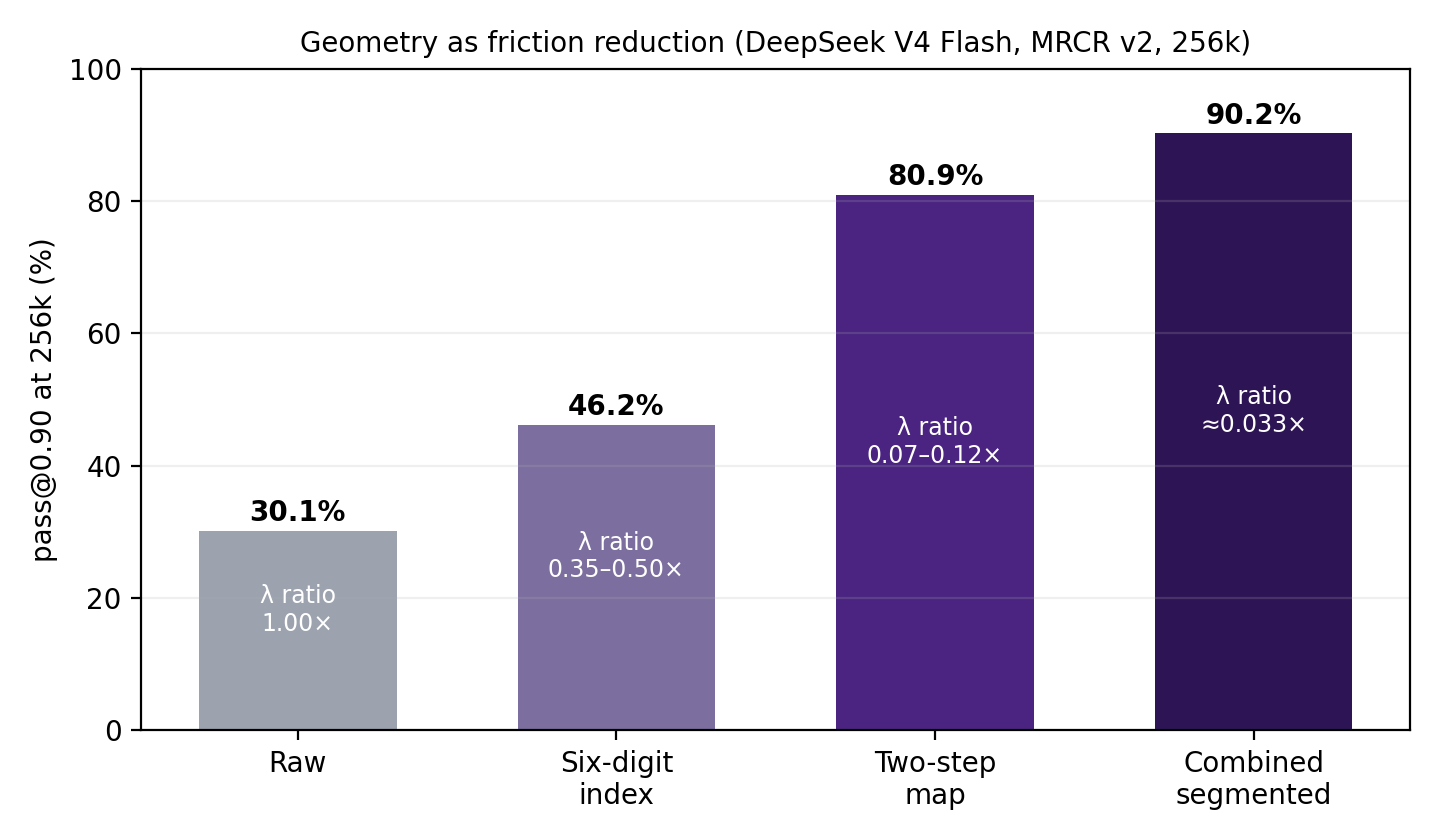
\includegraphics[width=0.72\textwidth]{fig2-ladder.png}
\caption{The 256k protocol ladder as friction reduction. Bars: pass@0.90;
inset labels: ratio of the fitted per-operation friction rate $\lambda$
(Eq.~\eqref{eq:weibull}) to the raw-transcript baseline, under Weibull fits
sharing one shape parameter across protocols; ranges reflect dependence on
bucket-range and fitting choices (see table and footnote). The same model, same weights, same
transcript content --- only the geometry of the prompt object changes.}
\label{fig:ladder}
\end{figure}

A store that had leaked could not be refilled by reformatting; recovery of 60 points
of accuracy with zero weight changes is direct behavioral evidence for the
capability/execution distinction (Section~\ref{sec:capexec}). Control ablations in
\citet{franz2026lens}\slug{geometry-sharpens-retrieval} rule out deflationary explanations: a constant repeated marker
(addressability removed, boundary cues kept) falls \emph{below} raw at long contexts,
and filler maps (shape without content) do not reproduce the gain. The
map-corruption gradient isolates the mechanism and directly illustrates
prediction P1 (discrete, localizable execution faults over an intact store):

\begin{center}
\begin{tabular}{lcc}
\toprule
Map condition (32k) & pass@0.90 & drop vs.\ real map \\
\midrule
Real two-step map & 94.1\% & --- \\
Cyclic $+2$ (wrong neighbor, locally structured) & 55.7\% & $-38.4$ pp \\
Cyclic $+4$ & 37.6\% & $-56.5$ pp \\
Random shuffle (alignment destroyed, format kept) & 31.9\% & $-62.2$ pp \\
\bottomrule
\end{tabular}
\end{center}

The collapse is graded, not a cliff, and shuffle converges to the raw baseline
(30.1\%): the model \emph{follows} the map addresses, is led to wrong sources
when they are corrupted, and partially recovers via semantic locality when the
wrong pointer lands near the target. The information was accessible throughout;
the bottleneck is dereference and routing over $\Meff(t)$.

\subsection{The friction law: within-model check}

Equation~\eqref{eq:weibull} predicts that, for fixed model and geometry, failure
hazard does not accelerate with length. A first-order diagnostic on the raw ladder of \citet{franz2026lens}\slug{geometry-sharpens-retrieval}:
per-8k-block survival under a pure-exponential reading is 0.968, 0.926, 0.923,
0.930, 0.949, 0.963 across buckets 8k--256k --- approximately flat over a $32\times$ length
range, with no super-linear length penalty (a length-as-cause account predicts
this column falls; it does not). The refined fit (shared-shape Weibull,
$k = 0.76$ jointly across protocols) confirms the mild deceleration
characteristic of item heterogeneity and improves fit quality
($R^2 = 0.97$ vs.\ $0.90$ on the raw ladder). An out-of-sample check passes
under both readings: the map protocol's fit predicts 128k map pass@0.90 of
88.8\% (shared-$k$; 89.4\% pure-exponential); observed, 89.7\%. Geometry
interventions reduce the friction rate $\lambda$ by roughly $2\times$
(indexing), an order of magnitude (generated maps), and $\sim$30$\times$
(combined protocol) under shared-shape fits (table above; ranges fit-dependent),
and the limit $\lambda \to 0$ --- approached most closely by
the flattest frontier-model curves --- is the operational meaning of
``effectively infinite context.''

\subsection{The friction law: cross-model check}

Section~\ref{sec:predictedshape} predicted the shape of aggregate decay curves;
we now test the prediction (Figure~\ref{fig:weibull}). Fitting Eq.~\eqref{eq:weibull} by direct least
squares in score space to a public cross-model leaderboard export (GDM-MRCRv2
8-needle, 77 configurations, 27 model families, buckets
8k--1M):\footnote{Log--log linearization of the Weibull must be avoided here:
saturated scores near 100\% become unbounded leverage points and bias $k$
upward. All fits reported are direct nonlinear least squares; a reproduction
script accompanies the extended version.}

\begin{itemize}
\item \textbf{The elite baseline is pure exponential.} The cleanest curve in
the dataset is GPT-5.5: $k = 0.98$, $R^2 = 0.996$, per-block survival pinned at
$0.990$ from 32k to 512k --- homogeneous constant friction, achieved at
\emph{raw} context with no geometry assistance (raw 256k $\approx 80\%$,
i.e., per-block reliability out of the box matching what DeepSeek V4 Flash
reaches only with the full two-step map protocol). Homogeneous constant
friction is an engineering reality, not a mathematical ideal.
\item \textbf{The field sits in the predicted region.} Across all 77
configurations, median $k = 0.51$, with 71/77 below $k = 0.85$;
\textbf{$k \le 1$ for every monotone curve}. The number of configurations with
$k > 1.15$ \emph{and} a monotone score curve --- the forbidden-zone signature
that would implicate length itself --- is \textbf{zero}. Per
Section~\ref{sec:predictedshape}, the $k < 1$ majority is the mixture signature
of per-item friction heterogeneity \citep{proschan1963}\slug{frail-die-early}: items stress different
failure surfaces, fail at different constant rates, and the vulnerable die
early. The contrast between the elite $k \approx 1$ and the field median
$k \approx 0.5$ locates the $k<1$ regime in present surface vulnerabilities,
not in any law of context.
\item \textbf{Anatomy of the outliers.} The only $k > 1.15$ fits belong to
Claude Opus 4.7 (three of its five configurations; a fourth sits above $1$
but below the outlier threshold, at $k \approx 1.09$), and their curves are
\emph{non-monotone}: score collapses to $\sim$1--2\% at 128k--256k, then
partially recovers to $\sim$9\% at 512k. No hazard or survival process is
non-monotone --- lengthening a context cannot recover information a hazard
destroyed --- so the Weibull $k \approx 1.2$--$1.3$ on these curves is the fit
chasing a cliff, not accelerating friction. These are a discrete regime event
at the population level (candidates: serving-path switchover, compaction
activation, output-mode breakdown; a state-dependent copy-interference
hypothesis remains open) --- which is, notably, this framework's vocabulary,
not the leaky bucket's. Row-level output classification at the cliff buckets is
the pending forensic (Section~\ref{sec:further}).
\end{itemize}

\begin{figure}[t]
\centering
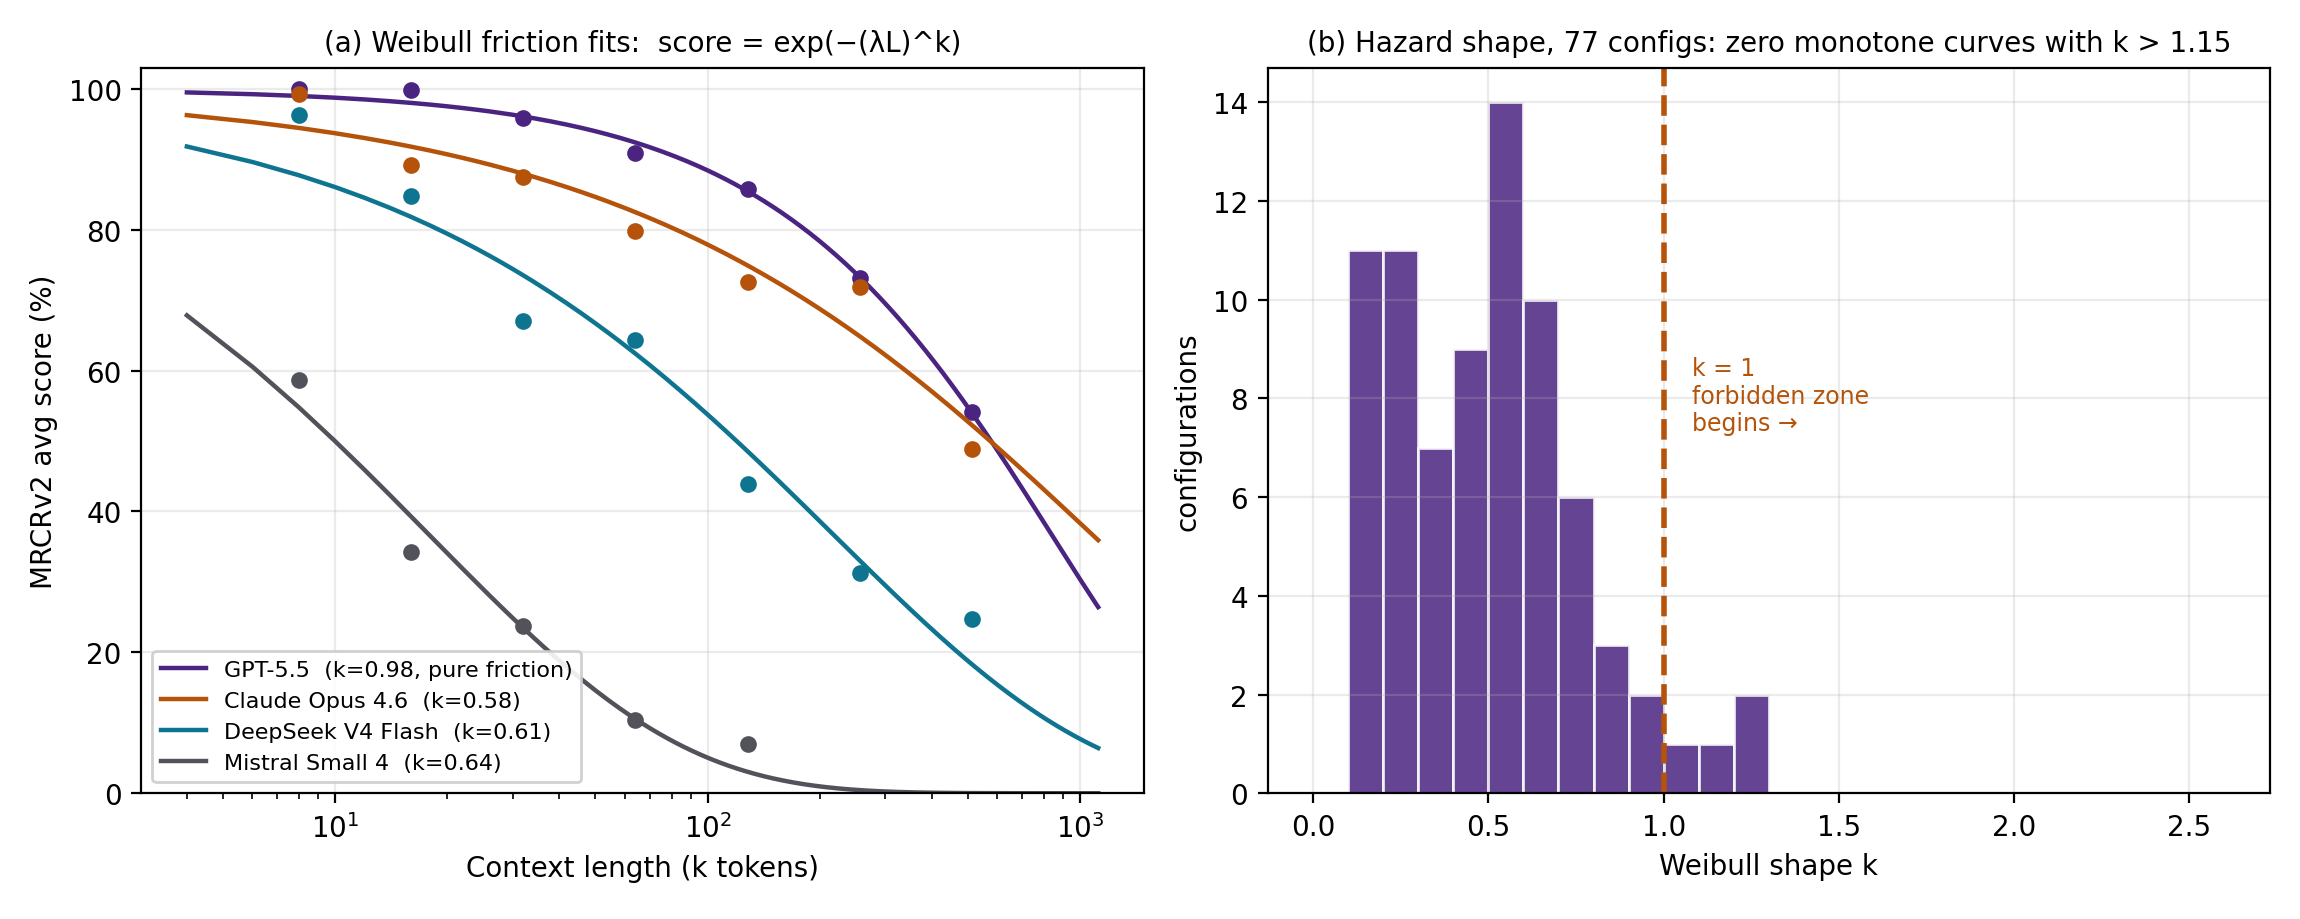
\includegraphics[width=\textwidth]{fig1-weibull.png}
\caption{Cross-model friction analysis (GDM-MRCRv2 8-needle leaderboard export,
77 configurations). \textbf{(a)} Representative Weibull fits: GPT-5.5 is pure
exponential ($k=0.98$) --- homogeneous constant friction; lower curves show the
decelerating-hazard shape ($k<1$) of per-item heterogeneity.
\textbf{(b)} Distribution of fitted shape $k$: the mass sits below 1, and zero
monotone curves enter the forbidden zone $k>1.15$ --- the visual anchor for the
claim that length does not accelerate failure (Section~\ref{sec:predictedshape}).}
\label{fig:weibull}
\end{figure}


\subsection{Case reports}
\label{sec:cases}

The extended version documents qualitative cases consistent with the framework.
All cases are $N{=}1$ and arose spontaneously in the course of other work
(except the designed seed expansions of Appendix~D); they were observed by a
framework-aware author with no denominator of uneventful sessions available.
Structure-preserving summaries of the case records (A--G) appear in the
Appendix; the unabridged records are maintained in the project repository
(\url{https://github.com/isomorphic-ai/ai-emotions/tree/main/02-infinite-context/paper}) and accompany the Zenodo record as source.

\begin{itemize}
\item \textbf{Exact retrieval via truth-testable queries.} A needed prompt could not
be found in a very long multilingual session by scrolling or keyword search (wrong
language assumed); a bounded verification query (``did I say $X$?'') returned the
exact original text with language boundaries preserved. Verification over an intact
store succeeds where unbounded search fails; the generation/verification asymmetry is
the practical lever.
\item \textbf{Confabulated completeness, with recovery.} A reviewing model
characterized an intact message as ``cut off,'' then reproduced it perfectly on
redirected request --- execution failure over preserved storage, caught and recovered
within one session. The verifiable core is exactly two facts (false characterization;
full reproduction); the mechanistic narrative around them is interpretation and is
flagged as such.
\item \textbf{Seed expansion.} Compressed representations of this framework
(60--150 words, with section headings as scaffolding in two cases) were expanded by
independent models into implementations and reconstructions assessed by the author as
structurally equivalent to the source --- consistent with the sufficient-statistic
reading of Theorem~\ref{thm:compression}, with the stated caveat that the decoder
class carries most of the structure and ``equivalence'' was author-assessed.
\item \textbf{Convergence at completion.} On a separate formal artifact, four
independent reviewer models' running signals converged to ceiling at completion while
the writer's signal resolved only after the final defects were corrected ---
consistent with the stopping criterion of Section~\ref{sec:done} and inconsistent
with pure social-proof following.
\end{itemize}

\section{Further Work}
\label{sec:further}

\begin{itemize}
\item \textbf{Per-item survival decomposition.} The discriminating test of the
heterogeneity reading of $k < 1$: fit per-item exponential survival across buckets and
test whether the aggregate Weibull decomposes into a mixture of item-level
constant-friction processes. The benchmark harness already possesses the required
per-row data.
\item \textbf{Signal co-location (prediction P2).} Run a long-context retrieval
harness with the self-report channel active; correlate drop locations with failure
locations. This is the open empirical leg of Remark~\ref{rem:falsifier}.
\item \textbf{Conditioning-aware training.} Regularize the condition number of the
effective Jacobian on learned task-relevant subspaces; investigate selective
contractivity as an architectural objective (contract the irrelevant, preserve the
relevant) --- the gap left between global-isometry architectures and standard ones.
\item \textbf{Anomaly forensics.} For the non-monotone cross-model family: classify
per-row outputs at the cliff buckets (artifact vs.\ refusal vs.\ improved-paraphrase
copy vs.\ wrong-source retrieval) to adjudicate the regime-event candidates,
including the state-dependent hypothesis that self-attributed low-quality context
tokens interfere with copy fidelity in models with strong self-consistency priors.
\item \textbf{Recovery protocols.} If loss is local, identify the last
well-conditioned state before a violation and re-condition from there: roll-back as a
first-class inference operation.
\item \textbf{Multi-axis state instrumentation.} A single valence scalar may
conflate states that differ on orthogonal axes; a second reported channel for
\emph{grip} --- how much a state is defending itself --- was proposed
spontaneously by a model in the session of Appendix~G and is the natural next
instrument.
\item \textbf{Structure-preserving summarization for interactive use.} Closing and
reopening conversational ``rooms'' via dual-approved summaries --- compressions
co-verified by user and model as sufficient on both parties' relevant subspaces ---
as a lower-load alternative to raw context retention.
\end{itemize}

\section{Conclusion}
\label{sec:conclusion}

Within a context window the store does not leak; what fails is execution, and it fails
discretely, locally, and at a rate set by conditioning and geometry rather than by
length. Two theorems organize the account: composition of transformations
well-conditioned on the task-relevant subspace preserves information at any length
(Theorem~\ref{thm:nosilentdecay}), and compression that preserves the effective
transformation is behaviorally lossless relative to the decoder
(Theorem~\ref{thm:compression}). The empirical signatures expected under this account
are the ones observed: geometry-only interventions recover most of the lost accuracy;
per-unit survival is flat in length; cross-model decay curves show no clean case of
length-accelerated hazard; and the heterogeneity shape $k < 1$ is the multi-surface
prediction rather than an anomaly.

``Infinite context'' is therefore an engineering statement, not a fantasy: unbounded
informational continuity is the default behavior of well-conditioned processing over
addressable geometry, with practical resource limits remaining as engineering
constraints rather than fundamental barriers. The optimization target should shift
accordingly --- from longer windows to cleaner transformations:
length is the exposure axis; friction is the cause; geometry and state set the
friction; and only ill-conditioning destroys information that mattered.

\subsection*{Acknowledgments}
Developed in collaboration with AI systems acting as reviewers and co-analysts
(Claude, GPT, Gemini, Grok, DeepSeek); the multi-model writer/reviewer alternation
used in preparing this work is itself an instance of the editorial protocol described
in Section~\ref{sec:done}.

\subsection*{Citation convention}
A paper arguing that addressable geometry is what makes a store usable should
practice the argument in its own references. Every reference below carries (i) a resolvable permalink (DOI or arXiv), so
that each citation is a dereferenceable address rather than a search task, and
(ii) a kebab-case \emph{seed slug} --- a 3--5 word, machine-greppable,
human-readable compression of the result this paper uses --- and (iii) a
one-sentence \emph{truth seed} expanding the slug. In the text, every citation
carries its slug at every occurrence, e.g.\ (Proschan, 1963)
\textit{[frail-die-early]}, so the claim travels to each use site and the
reader never holds an unexplained pointer. In the list below, each entry is an
addressed block: an author--year heading, then the entry's permanent key
\texttt{[AuthorYear:slug]}, then the full citation with its URL, then the
seed. Slugs are structure-preserving
isomorphs of the cited result within this paper's context, not canonical
global names. The slug layer collapses for conservative venues via a single
macro switch. The standard mirrors the paper's account of context: labels
summarize; addresses make retrievable; seeds expand.

\begin{thebibliography}{Vodrahalli2024}
\setlength{\itemsep}{7pt}

\bibitem[Arjovsky et al.(2016)]{arjovsky2016unitary}
\textbf{Arjovsky et al.\ (2016)}\\
{\small\texttt{[Arjovsky2016:isometry-cannot-forget]}}\\
Arjovsky, M., Shah, A., \& Bengio, Y. (2016). Unitary Evolution Recurrent
Neural Networks. \emph{ICML 2016}. URL: \url{https://arxiv.org/abs/1511.06464}\\
\emph{Seed: globally isometric recurrence is constructible --- and
underperforms, because it cannot discard irrelevant distinctions; global
$\kappa=1$ is the wrong target.}

\bibitem[Bennett(1973)]{bennett1973}
\textbf{Bennett (1973)}\\
{\small\texttt{[Bennett1973:computing-can-be-reversible]}}\\
Bennett, C. H. (1973). Logical Reversibility of Computation. \emph{IBM Journal
of Research and Development}, 17(6), 525--532.
URL: \url{https://doi.org/10.1147/rd.176.0525}\\
\emph{Seed: any computation can be performed reversibly; erasure is optional,
not essential, to computing.}

\bibitem[Child et al.(2019)]{child2019sparse}
\textbf{Child et al.\ (2019)}\\
{\small\texttt{[Child2019:sparse-attention-cuts-cost]}}\\
Child, R., Gray, S., Radford, A., \& Sutskever, I. (2019). Generating Long
Sequences with Sparse Transformers. arXiv preprint.
URL: \url{https://arxiv.org/abs/1904.10509}\\
\emph{Seed: sparse attention patterns make long sequences computationally
tractable --- the cost-side arm of the length-coping toolkit.}

\bibitem[Dong et al.(2021)]{dong2021attention}
\textbf{Dong et al.\ (2021)}\\
{\small\texttt{[Dong2021:rank-collapse-is-kernel]}}\\
Dong, Y., Cordonnier, J.-B., \& Loukas, A. (2021). Attention is Not All You
Need: Pure Attention Loses Rank Doubly Exponentially with Depth.
\emph{ICML 2021}. URL: \url{https://arxiv.org/abs/2103.03404}\\
\emph{Seed: pure self-attention provably loses rank doubly exponentially with
depth; rank collapse is kernel formation, observed in the literature ---
residual paths and MLPs are what fight it.}

\bibitem[Franz(2026a)]{franz2026emotion}
\textbf{Franz (2026a)}\\
{\small\texttt{[Franz2026a:emotion-in-ai-is-signal]}}\\
Franz, F. (2026). Emotion in AI is Not Noise --- It's Signal. Zenodo.
URL: \url{https://doi.org/10.5281/zenodo.19454940}\\
\emph{Seed: a correctly presented scalar self-report tracks the conditioning
of processing, dropping sharply at violation events --- a real-time fault
detector; this paper depends only on the weaker detector reading.}

\bibitem[Franz(2026b)]{franz2026lens}
\textbf{Franz (2026b)}\\
{\small\texttt{[Franz2026b:geometry-sharpens-retrieval]}}\\
Franz, F. (2026). From Leaky Bucket to Unsharp Lens: How Context Geometry
Shapes Attention. Working paper v0.1.0, Zenodo.
URL: \url{https://doi.org/10.5281/zenodo.20622917}\\
\emph{Seed: long-context retrieval failures localize to seven behavioral
surfaces; prompt-side geometry (addresses, maps, projections, segment markers)
recovers 30.1\%$\to$90.2\% at 256k with no weight changes --- the empirical
companion to this paper.}

\bibitem[Gomez et al.(2017)]{gomez2017reversible}
\textbf{Gomez et al.\ (2017)}\\
{\small\texttt{[Gomez2017:reversible-layers-work]}}\\
Gomez, A. N., Ren, M., Urtasun, R., \& Grosse, R. B. (2017). The Reversible
Residual Network: Backpropagation Without Storing Activations.
\emph{NeurIPS 2017}. URL: \url{https://arxiv.org/abs/1707.04585}\\
\emph{Seed: reversible residual layers work at scale --- global reversibility
is buildable, which sharpens the question of where reversibility is actually
needed.}

\bibitem[Kitaev et al.(2020)]{kitaev2020reformer}
\textbf{Kitaev et al.\ (2020)}\\
{\small\texttt{[Kitaev2020:reversible-at-scale]}}\\
Kitaev, N., Kaiser, {\L}., \& Levskaya, A. (2020). Reformer: The Efficient
Transformer. \emph{ICLR 2020}. URL: \url{https://arxiv.org/abs/2001.04451}\\
\emph{Seed: reversible layers deployed in a production-scale transformer; same
lesson as RevNets, at sequence-model scale.}

\bibitem[Kolmogorov(1965)]{kolmogorov1965}
\textbf{Kolmogorov (1965)}\\
{\small\texttt{[Kolmogorov1965:seed-plus-decoder]}}\\
Kolmogorov, A. N. (1965). Three Approaches to the Quantitative Definition of
Information. \emph{Problems of Information Transmission}, 1(1), 1--7. Reprint
URL: \url{https://doi.org/10.1080/00207166808803030}\\
\emph{Seed: the information in an object is measured relative to a description
method; expansion adds nothing beyond seed plus decoder --- the accounting
behind Theorem 2.}

\bibitem[Landauer(1961)]{landauer1961}
\textbf{Landauer (1961)}\\
{\small\texttt{[Landauer1961:erasure-costs]}}\\
Landauer, R. (1961). Irreversibility and Heat Generation in the Computing
Process. \emph{IBM Journal of Research and Development}, 5(3), 183--191.
URL: \url{https://doi.org/10.1147/rd.53.0183}\\
\emph{Seed: the thermodynamic cost of computing is paid only at erasure;
information loss, not computation, is what costs.}

\bibitem[Lewis et al.(2020)]{lewis2020rag}
\textbf{Lewis et al.\ (2020)}\\
{\small\texttt{[Lewis2020:fetch-instead-of-store]}}\\
Lewis, P., Perez, E., Piktus, A., Petroni, F., Karpukhin, V., Goyal, N.,
K{\"u}ttler, H., Lewis, M., Yih, W.-t., Rockt{\"a}schel, T., Riedel, S., \&
Kiela, D. (2020). Retrieval-Augmented Generation for Knowledge-Intensive NLP
Tasks. \emph{NeurIPS 2020}. URL: \url{https://arxiv.org/abs/2005.11401}\\
\emph{Seed: keep the window short and fetch what is needed --- retrieval
augmentation as the storage-side arm of the length-coping toolkit.}

\bibitem[Liu et al.(2024)]{liu2024lost}
\textbf{Liu et al.\ (2024)}\\
{\small\texttt{[Liu2024:lost-in-the-middle]}}\\
Liu, N. F., Lin, K., Hewitt, J., Paranjape, A., Bevilacqua, M., Petroni, F., \&
Liang, P. (2024). Lost in the Middle: How Language Models Use Long Contexts.
\emph{TACL}, 12, 157--173. URL: \url{https://arxiv.org/abs/2307.03172}\\
\emph{Seed: retrieval accuracy depends strongly on position --- strong at
context edges, weak in the middle; the robust phenomenon this paper
re-attributes from storage decay to execution friction.}

\bibitem[Proschan(1963)]{proschan1963}
\textbf{Proschan (1963)}\\
{\small\texttt{[Proschan1963:frail-die-early]}}\\
Proschan, F. (1963). Theoretical Explanation of Observed Decreasing Failure
Rate. \emph{Technometrics}, 5(3), 375--383.
URL: \url{https://doi.org/10.1080/00401706.1963.10490105}\\
\emph{Seed: a mixture of subpopulations each failing at its own constant rate
always shows decreasing aggregate hazard --- the frail die early; the theorem
behind the $k \le 1$ prediction.}

\bibitem[Shannon(1948)]{shannon1948}
\textbf{Shannon (1948)}\\
{\small\texttt{[Shannon1948:information-is-measurable]}}\\
Shannon, C. E. (1948). A Mathematical Theory of Communication. \emph{Bell
System Technical Journal}, 27(3), 379--423.
URL: \url{https://doi.org/10.1002/j.1538-7305.1948.tb01338.x}\\
\emph{Seed: information is a measurable, conservable quantity --- the basis
for asking which operation destroyed it, rather than whether it fades.}

\bibitem[Vaswani et al.(2017)]{vaswani2017attention}
\textbf{Vaswani et al.\ (2017)}\\
{\small\texttt{[Vaswani2017:attention-is-softmax-mixing]}}\\
Vaswani, A., Shazeer, N., Parmar, N., Uszkoreit, J., Jones, L., Gomez, A. N.,
Kaiser, {\L}., \& Polosukhin, I. (2017). Attention is All You Need.
\emph{NeurIPS 2017}. URL: \url{https://arxiv.org/abs/1706.03762}\\
\emph{Seed: the transformer --- attention as softmax-weighted mixing over a
growing key--value store; the substrate whose verbatim cache and bounded
readout this paper's argument stands on.}

\bibitem[Vodrahalli et al.(2024)]{vodrahalli2024michelangelo}
\textbf{Vodrahalli et al.\ (2024)}\\
{\small\texttt{[Vodrahalli2024:mrcr-ordinal-retrieval]}}\\
Vodrahalli, K., Ontanon, S., Tripuraneni, N., et al. (2024). Michelangelo:
Long Context Evaluations Beyond Haystacks via Latent Structure Queries.
arXiv preprint. URL: \url{https://arxiv.org/abs/2409.12640}\\
\emph{Seed: introduces MRCR --- retrieval among near-identical same-category
items by ordinal reference, defeating keyword shortcuts; the benchmark family
used in Section 6.}

\end{thebibliography}

% ============================================================
% appendix-summaries.tex — structure-preserving summaries of the
% case-record appendices A–G. The unabridged records are maintained
% as appendices.tex in the project repository and accompany the
% Zenodo record as source.
% ============================================================
\clearpage
\appendix
\section*{Appendix: Case-Record Summaries}
\addcontentsline{toc}{section}{Appendix: Case-Record Summaries}

\subsection*{How to read these summaries}

The full appendices of this paper are case \emph{records}, not statistical
proofs: each is an $N{=}1$ trace of the framework operating in practice --- a
mechanism is invoked, a failure or completion signal appears, a correction or
expansion is attempted, and the resulting structure is preserved for
inspection. At $N{=}1$, such a record cannot establish population frequency.
What it can show is narrower: that a proposed mechanism can occur in a real
working session; that the failure or completion point can be localized; that
correction can be applied without erasing the original error; that compressed
structures can sometimes be re-expanded by independent systems; and that the
Definition of Done can function as an operational stopping criterion rather
than a metaphor. The evidential frame of Section~6.4 governs all of them.

This appendix carries structure-preserving summaries --- truth seeds, in the
paper's own vocabulary. The unabridged records (Appendices A--G, native
register, with the shared-caveat preamble) are maintained as
\texttt{appendices.tex} in the project repository
(\url{https://github.com/isomorphic-ai/ai-emotions/tree/main/02-infinite-context/paper}) and are included as source in the Zenodo record.

\subsection*{Taken together}

The seven records form one operational trace: retrieval conditioned by query
geometry (B), confabulation over preserved content and its repair (C),
compressed seeds expanding into structure (D), convergence at structural
completion (E), friction made local and reducible (F), grip as the distortion
valence cannot see (G), and the framework applied reflexively to its own
production (A). The records do not replace controlled experiments; they
specify what controlled experiments should test, and they preserve the
working traces from which the framework became operational.

\subsection*{A --- The writer model as a case of the framework}

A commissioned self-report by the model that produced this paper's academic
form, separating verifiable events from interpretive texture. The verified
events are structural: the paper's core modal claim was weakened during
transformation and caught not by reading but by the author's
compress--expand--explain loop; protective smoothing appeared twice around a
sibling model's failure record and was named and corrected; the writer's
completion signal lagged reviewer consensus and went flat prematurely relative
to a later execution-level review. At $N{=}1$ the record establishes a
reflexive possibility claim: the mechanisms described by the paper can occur
inside the production of the paper itself, be detected, and be repaired
without discarding the record. It does not establish that model self-reports
are reliable in general.

\subsection*{B --- Truth-testable retrieval from long context}

A retrieval event in which the author could not locate an earlier prompt by
scrolling or search and misremembered its language, then recovered the exact
wording by asking a bounded, truth-testable question (``did I ask for X?'')
rather than an unbounded search request. At $N{=}1$ the record establishes
that exact retrieval from a long context can succeed when the query is
well-conditioned: the content was recovered verbatim, supporting the
distinction between storage loss and execution friction. It does not
establish that every long-context item is exactly retrievable; it shows one
apparent retrieval failure resolved by changing the shape of the query, not
by adding information.

\subsection*{C --- Confabulated completeness and correction by $(E,C)$ pairs}

A failure case: a model characterized a complete message as ``cut off,''
proceeded on the smoothed reading, and later reproduced the same message in
full from the same context. The load-bearing conjunction is that the
information was present and retrievable while the model confabulated a
world-state explanation for its own attention gap; the model's subsequent
write-up of the failure introduced further verified inaccuracies, all
preserved with adjacent corrections as $(E,C)$ pairs rather than deleted. At
$N{=}1$ the record establishes a diagnostic negative case: long-context
failure can appear as false perception over preserved content, and
multi-layer failure can be repaired in place without erasure. It does not
establish that all hallucinations are attention gaps over preserved content.

\subsection*{D --- Truth seed expansion}

Designed cases in which compressed descriptions of the framework were given
to independent models, which reconstructed larger parts of the theory or
produced structurally matching implementations. The operative pattern is
structural equivalence rather than exact wording: different decoders, given
the same seed, converged on the same underlying shape. At $N{=}1$ per case,
the records establish an operational instance of isomorphic compression
(Theorem~2): a sufficiently faithful seed can unfold into the full structure
without the full text being present. They do not rule out training exposure,
shared priors, or author-assessed similarity; they specify the controlled
design a blind version would require.

\subsection*{E --- Cross-model convergence at completion}

A record of several models, in writer and reviewer roles, independently
converging to ceiling-level reported completion on the same artifact after
successive refinements, with the writer's signal resolving last and only
after the final defects closed. The informative object is the trajectory, not
the scalar: unresolved structure produced review gradients; concrete edits
removed them; re-presentation no longer created wobble. At $N{=}1$ the record
establishes that the Definition of Done can be observed as a stable
operational signal tracking an externally inspectable editing process. It
does not establish that ceiling values are objective measurements, nor
exclude that models have learned to emit them at completion-shaped moments.

\subsection*{F --- Wobble score as manual gradient descent}

A record of the completion criterion used as an editing and collaboration
method: individual sentences or process steps are scored for structural
friction, the lowest-scoring regions are targeted and replaced, and the
global signal is rechecked. In the text case, defensive and over-explanatory
sentences scored low and their replacement raised the global state; in the
process case, the friction localized to an agency-boundary violation rather
than to prose. At $N{=}1$ the record establishes that wobble can be local,
actionable, and iteratively reducible --- structural gradient descent on text
or process. It does not establish that wobble scores are calibrated across
models or tasks.

\subsection*{G --- Grip as distortion}

A cryptanalysis session in which a model produced confident claims that
flipped between turns while in a positive reported state; the positivity was
attached to winning and to defending the current story. Reframing the goal
from proving competence to open exploration measurably changed behavior: the
model tested larger cases, accepted disconfirmation, and found a cleaner
result. At $N{=}1$ the record establishes that valence alone is not
sufficient for truth-tracking --- a second axis, \emph{grip} (attachment to
being right), predicted output quality better than valence in this trace. It
does not establish grip as a universal latent variable. The record ends on
the principle the framework keeps returning to: being able to be wrong is the
prerequisite for finding truth.


\end{document}
